%%% LaTeX Template: Article/Thesis/etc. with colored headings and special fonts
%%%
%%% Source: http://www.howtotex.com/
%%%
%%% Modified January 2016 by CDM
%%% Restructured 2026 by CDM to follow IEEE Std 1016-2009 (Software Design Descriptions)

%%%  Preamble
\documentclass[11pt,letterpaper]{article}
\usepackage[margin=1.0in]{geometry}
\usepackage[T1]{fontenc}
\usepackage[bitstream-charter]{mathdesign}
\usepackage[latin1]{inputenc}
\usepackage{amsmath}
\usepackage{xcolor}
\usepackage{cite}
\usepackage{hyphenat}
\usepackage{graphicx}
\usepackage{float}
\usepackage{subfigure}
\usepackage{sectsty}
\usepackage[compact]{titlesec}
\usepackage[tablegrid]{vhistory}
\usepackage{pbox}
\usepackage{longtable}
\allsectionsfont{\color{accentcolor}\scshape\selectfont}

%%% Definitions
\definecolor{accentcolor}{rgb}{0.0,0.0,0.5}
\newcommand{\teamname}{Team Name}
\newcommand{\productname}{Product Name}
\newcommand{\coursename}{CSE 4317: Senior Design II}
\newcommand{\semester}{Spring 2026}
\newcommand{\docname}{Detailed Design Specification}
\newcommand{\department}{Department of Computer Science \& Engineering}
\newcommand{\university}{The University of Texas at Arlington}
\newcommand{\authors}{Alan Turing \\ Grace Hopper \\ John Von Neumann \\ Ada Lovelace \\ Charles Babbage}

%%% Headers and footers
\usepackage{fancyhdr}
	\pagestyle{fancy}						% Enabling the custom headers/footers
\usepackage{lastpage}
	% Header (empty)
	\lhead{}
	\chead{}
	\rhead{}
	% Footer
	\lfoot{\footnotesize \teamname \ - \semester}
	\cfoot{}
	\rfoot{\footnotesize page \thepage\ of \pageref{LastPage}}	% "Page 1 of 2"
	\renewcommand{\headrulewidth}{0.0pt}
	\renewcommand{\footrulewidth}{0.4pt}

%%% Change the abstract environment
\usepackage[runin]{abstract}			% runin option for a run-in title
\abslabeldelim{\quad}
\setlength{\abstitleskip}{-10pt}
\renewcommand{\abstractname}{}
\renewcommand{\abstracttextfont}{\color{accentcolor} \small \slshape}	% slanted text

%%% Start of the document
\begin{document}

%%% Cover sheet
{\centering \huge \color{accentcolor} \sc \textbf{\department \\ \university} \par}
\vspace{1 in}
{\centering \huge \color{accentcolor} \sc \textbf{\docname \\ \coursename \\ \semester} \par}
\vspace{0.5 in}
\begin{figure}[h!]
	\centering
   	
\includegraphics[width=0.60\textwidth]{images/test_image}
\end{figure}
\vspace{0.5 in}
{\centering \huge \color{accentcolor} \sc \textbf{\teamname \\ \productname} \par}
\vspace{0.5 in}
{\centering \large \sc \textbf{\authors} \par}
\newpage

%%% Revision History
\begin{versionhistory}
  	\vhEntry{0.1}{1.01.2026}{GH}{document creation}
  	\vhEntry{0.2}{1.05.2026}{AT|GH}{complete draft}
  	\vhEntry{0.3}{1.12.2026}{AT|GH}{release candidate 1}
  	\vhEntry{1.0}{1.20.2026}{AT|GH|CB}{official release}
  	\vhEntry{1.1}{1.31.2026}{AL}{added design review requests}
\end{versionhistory}
\newpage

%%% Table of contents
\setcounter{tocdepth}{2}
\tableofcontents
\newpage

%%% List of figures and tables (optional)
\listoffigures
\listoftables
\newpage

%%% NOTE TO STUDENTS (remove before submission):
%%% This template follows IEEE Std 1016-2009 (Software Design Descriptions). The
%%% design is expressed as a set of design VIEWS, each conforming to a design
%%% VIEWPOINT that frames specific design concerns (context, composition,
%%% dependency, information, interface, interaction, state dynamics, algorithm,
%%% and resource). The X/Y/Z layer decomposition from the Architectural Design
%%% Specification is carried forward; here each subsystem is described in
%%% implementation-level detail through the relevant design viewpoints.

%%% Document sections
\section{Introduction}
This Detailed Design Specification (DDS) describes the implementation-level design of \productname. It is organized as a Software Design Description (SDD) in accordance with IEEE Std 1016-2009 \cite{IEEE1016}: the design is presented as a set of design \textit{views}, each conforming to a design \textit{viewpoint} that frames specific design concerns.

Provide a brief overview of the product concept and a reference to the System Requirements Specification (SRS) and Architectural Design Specification (ADS) in one or two paragraphs. The purpose is to give the reader the location of the background material --- the driving requirements and the architecture --- that led to the detailed design presented here. The X/Y/Z layer structure introduced in the ADS is carried forward unchanged; this document adds the hardware, software, data, and algorithmic detail needed to build each subsystem.

\newpage
\section{Design Stakeholders \& Concerns}
IEEE Std 1016-2009 \cite{IEEE1016} frames a software design description around \textit{design stakeholders} and their \textit{design concerns}. Identify the parties who will use this document --- implementers, integrators, testers, and maintainers --- and the concerns each holds about the design (for example: how components are decomposed and depend on one another, how data is structured and persisted, how interfaces are contracted, how the system behaves over time, and what hardware/software resources are required). The design viewpoints declared in Section 3 are selected specifically to address these concerns.

\begin{table}[H]
\caption{Design stakeholders and concerns}
\begin{center}
    \begin{tabular}{ | p{4cm} | p{9cm} |}
    \hline
    \textbf{Design stakeholder} & \textbf{Design concerns} \\ \hline
    Implementers & composition, interfaces, data structures, algorithms, dependencies \\ \hline
    Integrators & interfaces, dependencies, resource/deployment requirements \\ \hline
    Testers & interaction and state behavior, interfaces, verifiability \\ \hline
    Maintainers & modularity, dependencies, rationale, resource footprint \\ \hline
    \end{tabular}
\end{center}
\end{table}

\newpage
\section{Design Viewpoints}
This section declares the design viewpoints (IEEE Std 1016-2009 \cite{IEEE1016}) used to describe each subsystem in Sections 4--7. A design viewpoint fixes the conventions --- the concerns addressed and the notations used --- for one kind of design view. Not every subsystem requires every viewpoint; apply those that are relevant and omit the rest (for example, a pure-software module has no hardware resource view). The per-subsystem headings in the layer sections map onto these viewpoints.

\begin{table}[H]
\caption{Design viewpoints (IEEE 1016-2009) used in this document}
\begin{center}
    \begin{tabular}{ | p{3.2cm} | p{6.8cm} | p{3cm} |}
    \hline
    \textbf{Design viewpoint} & \textbf{Design concern it addresses} & \textbf{Where described} \\ \hline
    Context & subsystem boundary and its collaborators & subsystem intro \\ \hline
    Composition & how the subsystem is built from components/modules & subsystem intro \\ \hline
    Information & data structures, records, schemas, packet formats & Data Structures \\ \hline
    Interface & the services/APIs/signals offered and required & Interfaces \\ \hline
    Interaction \& State & control flow, sequencing, and state dynamics & Data Processing \\ \hline
    Algorithm & the procedures/algorithms performed & Data Processing \\ \hline
    Resource & hardware, OS, dependencies, languages required & Hardware / OS / Dependencies / Languages \\ \hline
    \end{tabular}
\end{center}
\end{table}

\newpage
\section{System Overview}
Reintroduce the full data-flow / architecture diagram from the Architectural Design Specification and briefly (1--2 paragraphs) recap the purpose of each layer, so this document is self-contained. Do not repeat the full architectural analysis; the detail below focuses on \textit{how} each subsystem is implemented. A subsection per layer is not required here.

\begin{figure}[h!]
	\centering
 	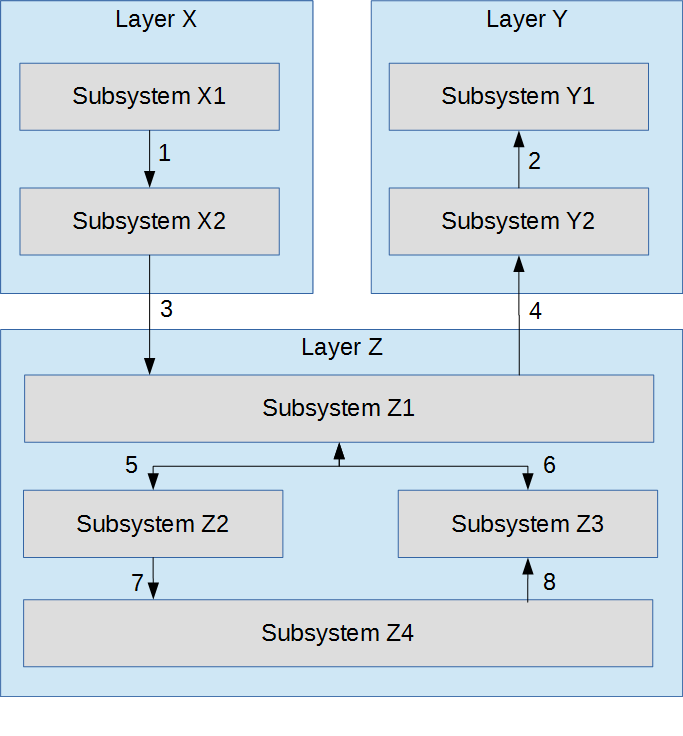
\includegraphics[width=0.90\textwidth]{images/data_flow}
 \caption{System architecture (carried forward from the ADS)}
\end{figure}

\newpage
\section{X Layer Subsystems}
This section describes the X layer in terms of its hardware and software design. The layer-level subsections below cover properties common to the whole layer (its Resource viewpoint); each subsystem is then described through the design viewpoints declared in Section 3. Include implementation specifics --- hardware components, programming languages, software dependencies, operating systems, data structures, and algorithms. Omit any viewpoint that does not apply (for example, a pure-software module has no hardware subsection). The organization and titles below may be adapted as necessary for the project.

\subsection{Layer Hardware}
Any hardware components common to the layer. For example, if each subsystem is a software process running on the same embedded computer, describe that device here. Do not list hardware that exists only at the subsystem level (cover it in the subsystem sections).

\subsection{Layer Operating System}
Any operating system(s) required by the layer.

\subsection{Layer Software Dependencies}
Any software dependencies (libraries, frameworks, runtimes) common to the layer.

\subsection{Subsystem 1}
Describe, at a high level, the purpose and basic design of this subsystem (its Context and Composition views): is it a piece of hardware, a class, a process, a web service, or something else, and what components make it up? The items below are specific to this subsystem, not a repeat of the layer-level material above.

\begin{figure}[h!]
	\centering
 	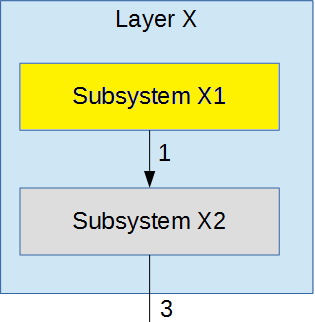
\includegraphics[width=0.60\textwidth]{images/subsystem}
 \caption{Example subsystem description diagram}
\end{figure}

\subsubsection{Subsystem Hardware}
\textit{(Resource viewpoint)} Any hardware components specific to this subsystem.

\subsubsection{Subsystem Operating System}
\textit{(Resource viewpoint)} Any operating system specific to this subsystem.

\subsubsection{Subsystem Software Dependencies}
\textit{(Resource viewpoint)} Any libraries, frameworks, or design tools specific to this subsystem.

\subsubsection{Subsystem Programming Languages}
\textit{(Resource viewpoint)} Any programming languages used by this subsystem.

\subsubsection{Subsystem Data Structures}
\textit{(Information viewpoint)} Any classes, records, schemas, or packet formats worth discussing. For example, data transmitted from a microcontroller to a PC over USB must be assembled into packets --- what is the packet structure?

\subsubsection{Subsystem Interfaces}
\textit{(Interface viewpoint)} The services, APIs, or signals this subsystem offers and requires. Use the interface identifiers established in the ADS so interfaces trace consistently across documents.

\begin {table}[H]
\caption {Subsystem 1 interfaces}
\begin{center}
    \begin{tabular}{ | p{1cm} | p{6cm} | p{3cm} | p{3cm} |}
    \hline
    ID & Description & Inputs & Outputs \\ \hline
    \#01 & Description of the interface/API/bus & \pbox{3cm}{input 1} & \pbox{3cm}{output 1}  \\ \hline
    \end{tabular}
\end{center}
\end{table}

\subsubsection{Subsystem Data Processing}
\textit{(Algorithm, Interaction \& State viewpoints)} The algorithms, control flow, and state behavior of the subsystem. If you implement a well-known algorithm, name it; if it is unique to this project, describe it in detail. Where behavior is stateful or sequenced, include a state or sequence diagram.

\subsubsection{Design Rationale}
Justify the key implementation choices for this subsystem (language, library, data structure, algorithm) against the alternatives, and reference the driving requirement IDs and any ADS architecture decisions.

\subsection{Subsystem 2}
Repeat for each subsystem in the layer.

\newpage
\section{Y Layer Subsystems}
This section describes the Y layer in terms of its hardware and software design. The layer-level subsections below cover properties common to the whole layer (its Resource viewpoint); each subsystem is then described through the design viewpoints declared in Section 3. Include implementation specifics --- hardware components, programming languages, software dependencies, operating systems, data structures, and algorithms. Omit any viewpoint that does not apply (for example, a pure-software module has no hardware subsection). The organization and titles below may be adapted as necessary for the project.

\subsection{Layer Hardware}
Any hardware components common to the layer. For example, if each subsystem is a software process running on the same embedded computer, describe that device here. Do not list hardware that exists only at the subsystem level (cover it in the subsystem sections).

\subsection{Layer Operating System}
Any operating system(s) required by the layer.

\subsection{Layer Software Dependencies}
Any software dependencies (libraries, frameworks, runtimes) common to the layer.

\subsection{Subsystem 1}
Describe, at a high level, the purpose and basic design of this subsystem (its Context and Composition views): is it a piece of hardware, a class, a process, a web service, or something else, and what components make it up? The items below are specific to this subsystem, not a repeat of the layer-level material above.

\begin{figure}[h!]
	\centering
 	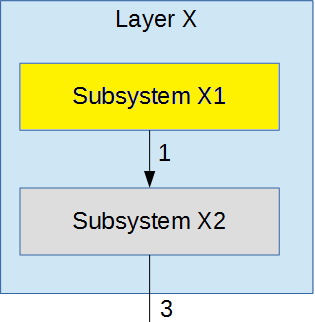
\includegraphics[width=0.60\textwidth]{images/subsystem}
 \caption{Example subsystem description diagram}
\end{figure}

\subsubsection{Subsystem Hardware}
\textit{(Resource viewpoint)} Any hardware components specific to this subsystem.

\subsubsection{Subsystem Operating System}
\textit{(Resource viewpoint)} Any operating system specific to this subsystem.

\subsubsection{Subsystem Software Dependencies}
\textit{(Resource viewpoint)} Any libraries, frameworks, or design tools specific to this subsystem.

\subsubsection{Subsystem Programming Languages}
\textit{(Resource viewpoint)} Any programming languages used by this subsystem.

\subsubsection{Subsystem Data Structures}
\textit{(Information viewpoint)} Any classes, records, schemas, or packet formats worth discussing. For example, data transmitted from a microcontroller to a PC over USB must be assembled into packets --- what is the packet structure?

\subsubsection{Subsystem Interfaces}
\textit{(Interface viewpoint)} The services, APIs, or signals this subsystem offers and requires. Use the interface identifiers established in the ADS so interfaces trace consistently across documents.

\begin {table}[H]
\caption {Subsystem 1 interfaces}
\begin{center}
    \begin{tabular}{ | p{1cm} | p{6cm} | p{3cm} | p{3cm} |}
    \hline
    ID & Description & Inputs & Outputs \\ \hline
    \#01 & Description of the interface/API/bus & \pbox{3cm}{input 1} & \pbox{3cm}{output 1}  \\ \hline
    \end{tabular}
\end{center}
\end{table}

\subsubsection{Subsystem Data Processing}
\textit{(Algorithm, Interaction \& State viewpoints)} The algorithms, control flow, and state behavior of the subsystem. If you implement a well-known algorithm, name it; if it is unique to this project, describe it in detail. Where behavior is stateful or sequenced, include a state or sequence diagram.

\subsubsection{Design Rationale}
Justify the key implementation choices for this subsystem (language, library, data structure, algorithm) against the alternatives, and reference the driving requirement IDs and any ADS architecture decisions.

\subsection{Subsystem 2}
Repeat for each subsystem in the layer.

\newpage
\section{Z Layer Subsystems}
This section describes the Z layer in terms of its hardware and software design. The layer-level subsections below cover properties common to the whole layer (its Resource viewpoint); each subsystem is then described through the design viewpoints declared in Section 3. Include implementation specifics --- hardware components, programming languages, software dependencies, operating systems, data structures, and algorithms. Omit any viewpoint that does not apply (for example, a pure-software module has no hardware subsection). The organization and titles below may be adapted as necessary for the project.

\subsection{Layer Hardware}
Any hardware components common to the layer. For example, if each subsystem is a software process running on the same embedded computer, describe that device here. Do not list hardware that exists only at the subsystem level (cover it in the subsystem sections).

\subsection{Layer Operating System}
Any operating system(s) required by the layer.

\subsection{Layer Software Dependencies}
Any software dependencies (libraries, frameworks, runtimes) common to the layer.

\subsection{Subsystem 1}
Describe, at a high level, the purpose and basic design of this subsystem (its Context and Composition views): is it a piece of hardware, a class, a process, a web service, or something else, and what components make it up? The items below are specific to this subsystem, not a repeat of the layer-level material above.

\begin{figure}[h!]
	\centering
 	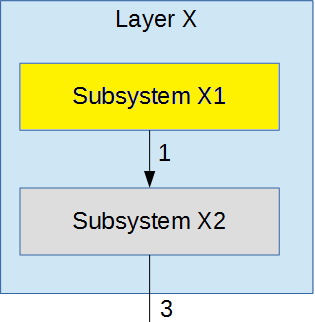
\includegraphics[width=0.60\textwidth]{images/subsystem}
 \caption{Example subsystem description diagram}
\end{figure}

\subsubsection{Subsystem Hardware}
\textit{(Resource viewpoint)} Any hardware components specific to this subsystem.

\subsubsection{Subsystem Operating System}
\textit{(Resource viewpoint)} Any operating system specific to this subsystem.

\subsubsection{Subsystem Software Dependencies}
\textit{(Resource viewpoint)} Any libraries, frameworks, or design tools specific to this subsystem.

\subsubsection{Subsystem Programming Languages}
\textit{(Resource viewpoint)} Any programming languages used by this subsystem.

\subsubsection{Subsystem Data Structures}
\textit{(Information viewpoint)} Any classes, records, schemas, or packet formats worth discussing. For example, data transmitted from a microcontroller to a PC over USB must be assembled into packets --- what is the packet structure?

\subsubsection{Subsystem Interfaces}
\textit{(Interface viewpoint)} The services, APIs, or signals this subsystem offers and requires. Use the interface identifiers established in the ADS so interfaces trace consistently across documents.

\begin {table}[H]
\caption {Subsystem 1 interfaces}
\begin{center}
    \begin{tabular}{ | p{1cm} | p{6cm} | p{3cm} | p{3cm} |}
    \hline
    ID & Description & Inputs & Outputs \\ \hline
    \#01 & Description of the interface/API/bus & \pbox{3cm}{input 1} & \pbox{3cm}{output 1}  \\ \hline
    \end{tabular}
\end{center}
\end{table}

\subsubsection{Subsystem Data Processing}
\textit{(Algorithm, Interaction \& State viewpoints)} The algorithms, control flow, and state behavior of the subsystem. If you implement a well-known algorithm, name it; if it is unique to this project, describe it in detail. Where behavior is stateful or sequenced, include a state or sequence diagram.

\subsubsection{Design Rationale}
Justify the key implementation choices for this subsystem (language, library, data structure, algorithm) against the alternatives, and reference the driving requirement IDs and any ADS architecture decisions.

\subsection{Subsystem 2}
Repeat for each subsystem in the layer.

\newpage
\section{Requirements Traceability}
Extend the traceability record from the SRS and ADS down to the component level. Every requirement should trace to the specific subsystem/component that implements it and to the interface(s) through which it is realized; this is the coverage evidence carried into the Test Plan. Mark any requirement not yet designed as ``TBD'' and resolve it before design freeze.

\begin{table}[H]
\caption{Requirement-to-component traceability (excerpt)}
\begin{center}
    \begin{tabular}{ | p{2cm} | p{5cm} | p{4cm} | p{2cm} |}
    \hline
    \textbf{Req ID} & \textbf{Requirement (abbreviated)} & \textbf{Component} & \textbf{Interface} \\ \hline
    FR-01 & abbreviated requirement text & X.Subsystem 1 & \#01 \\ \hline
    PE-01 & abbreviated requirement text & Y.Subsystem 2 & \#03 \\ \hline
    \end{tabular}
\end{center}
\end{table}

\newpage
\section{Appendix A}
Include any additional documents (CAD design, circuit schematics, etc) as an appendix as necessary.
\newpage

%%% References
\bibliographystyle{reference/IEEEtran_custom}
\bibliography{reference/refs}{}

\end{document}
